\documentclass{beamer}

\usepackage{multirow}
\usepackage{subcaption}
\usepackage{mathtools}
\usepackage{amsmath}
\usepackage{amssymb}
\usepackage{amsbsy}
\usepackage{graphicx}
\usepackage{xfrac}
\usepackage{xcolor}
\usepackage{cancel}
\usepackage{overpic}
\usepackage{sidecap}
\usepackage[sfdefault]{atkinson}
\usepackage[T1]{fontenc}
\usepackage{etoolbox}
\usepackage{ragged2e}
\let\raggedright\justifying

\newcommand\todo[1]{{\textcolor{red}{#1}}}
\DeclareMathOperator*{\argmin}{arg\,min}
\DeclareMathOperator*{\argmax}{arg\,max}

%Arquivo com ajustes padrões para gerar slides no beamer com as cores e logo da UFV.

\usetheme{CambridgeUS}
\usepackage[T1]{fontenc}      %caracteres corretos na saída em pdf
\usepackage[utf8]{inputenc}   % fontes com acentos
% \usepackage[brazil]{babel}    % português do Brasil.
\usepackage{lmodern}
\usepackage{url}

\usepackage{csquotes}
\usepackage{booktabs}

\usepackage{listings} % Para exibir codigo fonte
\usepackage{lstautogobble}
\usepackage[scaled]{beramono} %fonte de tamanho fixo mais bonita para o código-fonte nos listings
\usepackage{textcomp} % Ajeitar os apóstrofos no código fonte para ficarem retos

\usepackage[backend=biber,style=numeric, citestyle=ieee]{biblatex}
% \usepackage[url=false,isbn=false,backend=biber]{biblatex}
% \usepackage[style=abnt, url=false, isbn=false,indent, noslsn,backend=biber]{biblatex}
\addbibresource{refs.bib}

\setbeamertemplate{bibliography item}{\insertbiblabel}

\usepackage[normalem]{ulem}% usar diferentes tipos de underline
    %\uline{important} underlined text
    %\uuline{urgent} double-underlined
    %\uwave{boat} wavy underline
    %\sout{wrong} line struck
    %\xout{removed} marked
    %\dashuline{dashing} dashed underline
    %\dotuline{dotty} dotted underline


\graphicspath{{logos_ufv/}}

%Logo da UFV
\titlegraphic{
\includegraphics[width=3.5cm]{logos_ufv/LogoSIN.png}}

\newcommand{\transparente}{\setbeamercovered{transparent}}
\newcommand{\invisivel}{\setbeamercovered{invisible}}
\newcommand{\destacar}[1]{\alert{#1}}


%Retirar ícones das bibliografias
\setbeamertemplate{bibliography item}{-}
%Notas de rodapé com fonte menor
\setbeamerfont{footnote}{size=\tiny}
%retirar os controles de navegação que ficam no canto inferior direito
\setbeamertemplate{navigation symbols}{}

%Cores do logo da UFV
\definecolor{ufvred}{RGB}{124,26,29}
\definecolor{ufvyellow}{RGB}{203,176,49}
\definecolor{DarkGray}{RGB}{118,118,118}
\definecolor{LightGray}{RGB}{214,214,206}

% format de círculo flat para os bullets...
\setbeamertemplate{itemize items}[circle]
% .. vermelhos
\usecolortheme[named={ufvred}]{structure}

%ajusta as cores dos elementos dos slides
% cor do título
\setbeamercolor{frametitle}{fg=ufvred}
\setbeamercolor{title}{fg=ufvred}
\setbeamercolor{subtitle}{fg=ufvred}

% parte do rodapé
\setbeamercolor{author in head/foot}{bg=black}
\setbeamercolor{title in head/foot}{bg=ufvred, fg=white}
\setbeamercolor{date in head/foot}{bg=ufvyellow, fg=black}
\setbeamercolor{section in head/foot}{bg=black, fg=white}
\setbeamercolor{subsection in head/foot}{bg=black, fg=white}

%=====================
% cores dos blocos
%=====================
% block
% \setbeamercolor{block title}{fg=ufvred}
% exampleblock
\setbeamercolor{block title}{fg=white, bg=DarkGray}
\setbeamercolor{block body}{bg=LightGray}
% \AtBeginEnvironment{exampleblock}{\setbeamercolor{itemize item}{fg=ufvred}}

% alertbox
\setbeamercolor{block title alerted}{fg=ufvred, bg=ufvyellow}
\setbeamercolor{block body alerted}{bg=ufvyellow!50}

% % block
% \setbeamercolor{block title}{fg=ufvred}
% % exampleblock
% \setbeamercolor{block title example}{fg=white, bg=DarkGray}
% \setbeamercolor{block body example}{bg=LightGray}
% \AtBeginEnvironment{exampleblock}{\setbeamercolor{itemize item}{fg=ufvred}}

% % alertbox
% \setbeamercolor{block title alerted}{fg=ufvred, bg=ufvyellow}
% \setbeamercolor{block body alerted}{bg=ufvyellow!50}

%Tamanho da fonte das referências
\renewcommand*{\bibfont}{\footnotesize}

\definecolor{dkgreen}{rgb}{0,0.6,0}

%======================
% Definições para exibição de código-fonte
%======================

\lstdefinestyle{SQL-Smarzaro}{%
	language=SQL,
	showspaces=false,
	basicstyle=\small\ttfamily,
	%    numbers=left,
	numberstyle=\tiny,
	commentstyle=\color{dkgreen},
	upquote=true,
	breaklines=true,
	morekeywords={*,REFERENCES,RENAME,TO,DATABASE,SCHEMA,IF,USE,REPLACE,REFRESH,MATERIALIZED,
		BEFORE, AFTER, INSTEAD, OF, FOR, EACH, ROW, DO, STATEMENT, RULE, FUNCTION, PROCEDURE...},
	keywordstyle=\color{blue}\bfseries,
	%frame=ltrb,
	backgroundcolor=\color{gray!20},
	inputencoding=latin1,
	extendedchars=true,
	autogobble=true,
    escapeinside={(*}{*)},          % if you want to add LaTeX within your code
}

\lstdefinestyle{TeX-Smarzaro}{language=[LaTeX]TeX,
	morekeywords={frame, fragile},
	keywordstyle=\color{blue}\bfseries,}
	
\lstset{style=SQL-Smarzaro,
	literate=
	{á}{{\'a}}1 {é}{{\'e}}1 {í}{{\'i}}1 {ó}{{\'o}}1 {ú}{{\'u}}1
	{Á}{{\'A}}1 {É}{{\'E}}1 {Í}{{\'I}}1 {Ó}{{\'O}}1 {Ú}{{\'U}}1
	{à}{{\`a}}1 {è}{{\`e}}1 {ì}{{\`i}}1 {ò}{{\`o}}1 {ù}{{\`u}}1
	{À}{{\`A}}1 {È}{{\'E}}1 {Ì}{{\`I}}1 {Ò}{{\`O}}1 {Ù}{{\`U}}1
	{ä}{{\"a}}1 {ë}{{\"e}}1 {ï}{{\"i}}1 {ö}{{\"o}}1 {ü}{{\"u}}1
	{Ä}{{\"A}}1 {Ë}{{\"E}}1 {Ï}{{\"I}}1 {Ö}{{\"O}}1 {Ü}{{\"U}}1
	{â}{{\^a}}1 {ê}{{\^e}}1 {î}{{\^i}}1 {ô}{{\^o}}1 {û}{{\^u}}1
	{Â}{{\^A}}1 {Ê}{{\^E}}1 {Î}{{\^I}}1 {Ô}{{\^O}}1 {Û}{{\^U}}1
	{Ã}{{\~A}}1 {ã}{{\~a}}1 {Õ}{{\~O}}1 {õ}{{\~o}}1
	{œ}{{\oe}}1 {Œ}{{\OE}}1 {æ}{{\ae}}1 {Æ}{{\AE}}1 {ß}{{\ss}}1
	{ű}{{\H{u}}}1 {Ű}{{\H{U}}}1 {ő}{{\H{o}}}1 {Ő}{{\H{O}}}1
	{ç}{{\c c}}1 {Ç}{{\c C}}1 {ø}{{\o}}1 {å}{{\r a}}1 {Å}{{\r A}}1
	{€}{{\euro}}1 {£}{{\pounds}}1 {«}{{\guillemotleft}}1
	{»}{{\guillemotright}}1 {ñ}{{\~n}}1 {Ñ}{{\~N}}1 {¿}{{?`}}1
}




\title{ORDER - Crop Mapping Anomaly Detection}
\subtitle{using Generative Models}
\author[Mateus Pinto da Silva]{\texorpdfstring{\logo \\ Mateus Pinto da Silva\\ \texttt{mateus.p.silva@ufv.br}}{Mateus Pinto da Silva}}
\institute[DPI - UFV]{Programa de Pós-Graduação em Ciência da Computação\\Universidade Federal de Viçosa}
\date{2026}

\newcommand{\currprop}{0.6\textheight}

\begin{document}

\invisivel

\AtBeginSection[]
{
    \begin{frame}<beamer>
        \frametitle{Summary}
        \tableofcontents[currentsection]
    \end{frame}
}

\frame{\titlepage}

\section{Introduction}
\label{sec:01:intro}

\renewcommand{\currprop}{0.8\textwidth}

\begin{frame}{The Challenges}
    \begin{itemize}
        \item Expert data labeling for RS is highly expensive. Conversely, free public maps (like MapBiomas or USDA CDL) often contain noisy or inconsistent labels.
        \pause
        \item The complexity increases with the size and heterogeneity of Satellite Image Time Series (SITS).
        \pause
        \item Modern Deep Neural Networks suffer from overconfidence: they exhibit high certainty even in incorrect predictions.
    \end{itemize}
\end{frame}

\begin{frame}{The Proposed Solutions}
    \begin{itemize}
        \item Instead of just improving models, \textbf{DCAI} focuses on improving data quality. We can apply rigorous filtering to noisy public labels to create highly reliable datasets.
        \pause
        \item The amount of public RS data is massive. \textbf{SSL} extracts patterns from this unlabeled data to generate supervisory signals.
        \pause
        \item To address overconfidence, we can treat incorrect predictions as anomalies in the model's embedding space. We propose \textbf{ORDER} (Open-set Recognition for Discriminative Error Rebuttal), a post-processing strategy using Gaussian Mixture Models (GMMs) to separate correct from incorrect predictions dynamically.
    \end{itemize}
\end{frame}

\section{Data Acquisition, SITS Datasets and Preprocessing}

\begin{frame}{The Proposed SITS Datasets}
    \begin{block}{Three Novel Parcel-Level Datasets}
        We generated three datasets: \textbf{Texas} (7 classes), \textbf{California} (14 classes), and \textbf{Brazil} (10 classes).
    \end{block}
    \pause
    \begin{block}{The Complexity of the Brazilian Dataset}
        Unlike the US regions (mostly single-cycle monocultures), Brazil presents unique challenges:
        \begin{itemize}
            \item \textbf{Subcontinental scale:} High regional variability in planting schedules across different biomes.
            \item \textbf{Double/Triple Cropping ("Safrinha"):} The presence of secondary crops acts as spectral noise, since public maps (like MapBiomas) provide only the primary crop label.
            \item \textbf{Noise from crop source:} MapBiomas deals with land use and cover, not active agriculture. 
        \end{itemize}
    \end{block}
\end{frame}

\section{Methods for Learning from SITS Data}

\begin{frame}{Complete Training Pipeline Overview}
    \renewcommand{\currprop}{0.6\textheight}
    
    \begin{block}{Pretraining, Finetuning and Error Rebuttal}
        \only<1| handout:0>{During the training stage, we first retrieve the unlabeled SITS samples.}
        \only<2| handout:0>{Samples have already been downloaded in the previous flow using our library.}
        \only<3| handout:0>{These samples undergo data augmentation to self-supervisedly pre-train the model using SSL strategies.}
        \only<4| handout:0>{The pre-trained backbone is then fine-tuned using a smaller, curated set of labeled samples.}
        \only<5| handout:0>{Using these fine-tuned embeddings, we train a distinct Gaussian Mixture Model (GMM) per class for the ORDER anomaly detection framework.}
        \only<6| handout:0>{In the inference stage, the standalone classifier makes an initial class prediction based on the time series.}
        \only<7| handout:1>{ORDER GMM pipeline verifies the prediction, acting as a critical gatekeeper to confirm or reject the classifier's output.}
    \end{block}
	\begin{figure}
		\centering
		\includegraphics<1| handout:0>[height=\currprop]{figures_slides/meth_graphical_abstract-6.pdf}
		\includegraphics<2| handout:0>[height=\currprop]{figures_slides/meth_graphical_abstract-6-marked.jpg}
		\includegraphics<3| handout:0>[height=\currprop]{figures_slides/meth_graphical_abstract-5.pdf}
		\includegraphics<4| handout:0>[height=\currprop]{figures_slides/meth_graphical_abstract-4.pdf}
		\includegraphics<5| handout:0>[height=\currprop]{figures_slides/meth_graphical_abstract-3.pdf}
		\includegraphics<6| handout:0>[height=\currprop]{figures_slides/meth_graphical_abstract-2.pdf}
        \includegraphics<7| handout:1>[height=\currprop]{figures_slides/meth_graphical_abstract-1.pdf}
	\end{figure}
\end{frame}

\begin{frame}{ORDER - In details}
    \renewcommand{\currprop}{0.5\textheight}
    
    \begin{block}{Open-set Recognition for Discriminative Error Rebutta}
        \only<1| handout:0>{The system utilizes the trainig and validation dataset to pass representations through the fine-tuned model backbone.}
        \only<2| handout:0>{Within the embedding space, the training samples initialize one distinct GMM for each crop class.}
        \only<3| handout:0>{Both positive and negative validation samples are subsequently mapped to evaluate these class boundaries.}
        \only<4| handout:0>{The hyperparameter optimization loop begins by scoring all validation sets against the fitted GMMs.}
        \only<5| handout:0>{This process actively maximizes the spatial separation between clean predictions and hard, out-of-distribution samples.}
        \only<6| handout:0>{A dynamic confidence threshold is statistically determined for each class by maximizing the F1-score.}
        \only<7| handout:0>{To ensure ultimate reliability, a conservative fallback mechanism (GEMOS) is integrated for cases with very few correct or incorrect validation samples.}
        \only<8| handout:0>{During class fixation, the system evaluates: 'Is the GMM score greater than the dynamic threshold?'}
        \only<9| handout:0>{At inference time, unseen time-series samples are projected into the classifier embedding space, as usual.}
        \only<10| handout:0>{The fine-tuned classification head assigns a preliminary label to the new inference sample.}
        \only<11| handout:1>{If the score exceeds the threshold, the prediction is trusted; otherwise, the sample is safely flagged as Unknown.}
    \end{block}
	\begin{figure}
		\centering
		\includegraphics<1| handout:0>[height=\currprop]{figures_slides/meth_models-10.pdf}
		\includegraphics<2| handout:0>[height=\currprop]{figures_slides/meth_models-9.pdf}
		\includegraphics<3| handout:0>[height=\currprop]{figures_slides/meth_models-8.pdf}
		\includegraphics<4| handout:0>[height=\currprop]{figures_slides/meth_models-7.pdf}
		\includegraphics<5| handout:0>[height=\currprop]{figures_slides/meth_models-6.pdf}
        \includegraphics<6| handout:0>[height=\currprop]{figures_slides/meth_models-5.pdf}
        \includegraphics<7| handout:0>[height=\currprop]{figures_slides/meth_models-4.pdf}
        \includegraphics<8| handout:0>[height=\currprop]{figures_slides/meth_models-3.pdf}
        \includegraphics<9| handout:0>[height=\currprop]{figures_slides/meth_models-2.pdf}
        \includegraphics<10| handout:0>[height=\currprop]{figures_slides/meth_models-1.pdf}
        \includegraphics<11| handout:1>[height=\currprop]{figures_slides/meth_models.pdf}
	\end{figure}
\end{frame}

\section{Experimental Setup}
\label{sec:06:setup}

\begin{frame}{Experimental Setup: Evaluation Scenarios \& Models}
    \begin{block}{Data Scarcity Regimes}
        To evaluate model robustness and the impact of Self-Supervised Learning, we simulated different label availability scenarios: \textbf{70\%} (traditional regime), \textbf{10\%}, \textbf{1\%}, and \textbf{0.1\%} (\textit{few-shot} regimes) of the training data \textbf{(RQ2)}.
    \end{block}
    
    \vspace{0.2cm}

    \begin{block}{Training Details}
        DL models were optimized using \textbf{AdamW}\footnote[1]{\url{https://arxiv.org/abs/1711.05101}} with a cosine annealing learning rate scheduler and Early Stopping. Conversely, SL models underwent Tree-structured Parzen Estimator\footnote[2]{\url{https://arxiv.org/abs/2304.11127}} hyperparameter search. 
    \end{block}
\end{frame}

\begin{frame}{Experimental Setup: Anomaly Detection (ORDER)}
    \begin{block}{Confidence Estimation Baselines}
        To evaluate the proposed \textbf{ORDER} \textbf{(RQ5)} method in detecting classification failures, we established two main baselines:
        \begin{itemize}
            \item \textbf{MCP (Maximum Class Probability):} The standard Softmax confidence.
            \item \textbf{ConfidNet:} An auxiliary neural network specifically trained to predict the True Class Probability (TCP) of the main classifier.
        \end{itemize}
    \end{block}

\end{frame}
    
\section{Results}

\subsection{Traditional Regime}

\begin{frame}{Traditional Regime}
    DL models (Transformers and Mamba) consistently outperform SL models with 70\% of labels without pretraining.
    
    \vspace{0.2cm}

    \begin{table}[h]
        \centering
        \resizebox{0.9\textwidth}{!}{
        \begin{tabular}{c|l|ccc}
        \hline
        \textbf{Type} & \textbf{Model} & \textbf{Brazil (F1)} & \textbf{Texas (F1)} & \textbf{California (F1)} \\ \hline
        \multirow{3}{*}{Shallow} & SVM & 77.7\% & 98.8\% & 97.2\% \\
         & Random Forest & 75.0\% & 97.9\% & 95.3\% \\
         & MLP & 79.2\% & 99.1\% & 97.0\% \\ \hline
        \multirow{4}{*}{Deep} & SITS-CNN & 83.8\% & 99.5\% & \textbf{98.2\%} \\
         & SITS-LSTM & 84.6\% & \textbf{99.6\%} & 97.4\% \\
         & SITS-BERT++ & \textbf{85.6\%} & 99.5\% & 97.7\% \\
         & SITS-Mamba & 85.0\% & \textbf{99.6\%} & 97.9\% \\ \hline
        \end{tabular}
        }
    \end{table}
\end{frame}

\subsection{Few Shot Regime}

\begin{frame}{Few Shot Regime}
    \begin{block}{The Impact of SSL in Data Scarcity}
        MoCo pre-training boosts F1-Scores by up to 40\% compared to random initialization.
    \end{block}

    \vspace{0.2cm}

    \begin{figure}
        \centering
        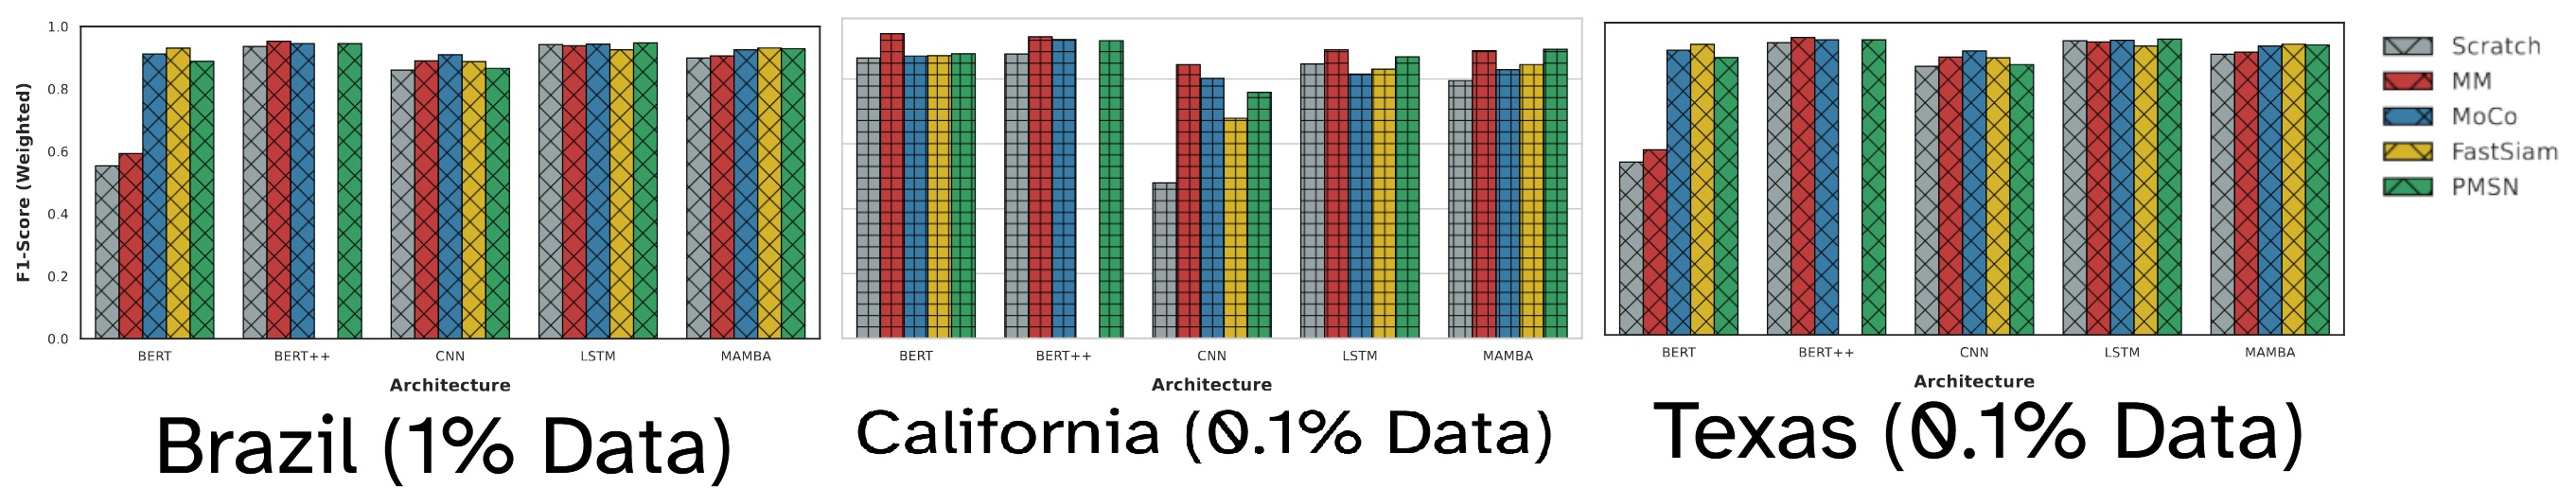
\includegraphics[width=\textwidth, keepaspectratio]{figures_slides/slide_few_shot.jpg}
    \end{figure}
    
\end{frame}

\begin{frame}{Anomaly Detection: The ORDER Method Overview}
    \begin{block}{Rebutting Classification Errors}
        Removing 5\% to 8\% of anomalies in Brazil raised the F1-Score from $\sim84\%$ to $\sim88\%$. In high-accuracy US regimes, ORDER acts remove far fewer samples. 
    \end{block}
    
    \vspace{0.2cm}
    
    \begin{figure}
        \centering
        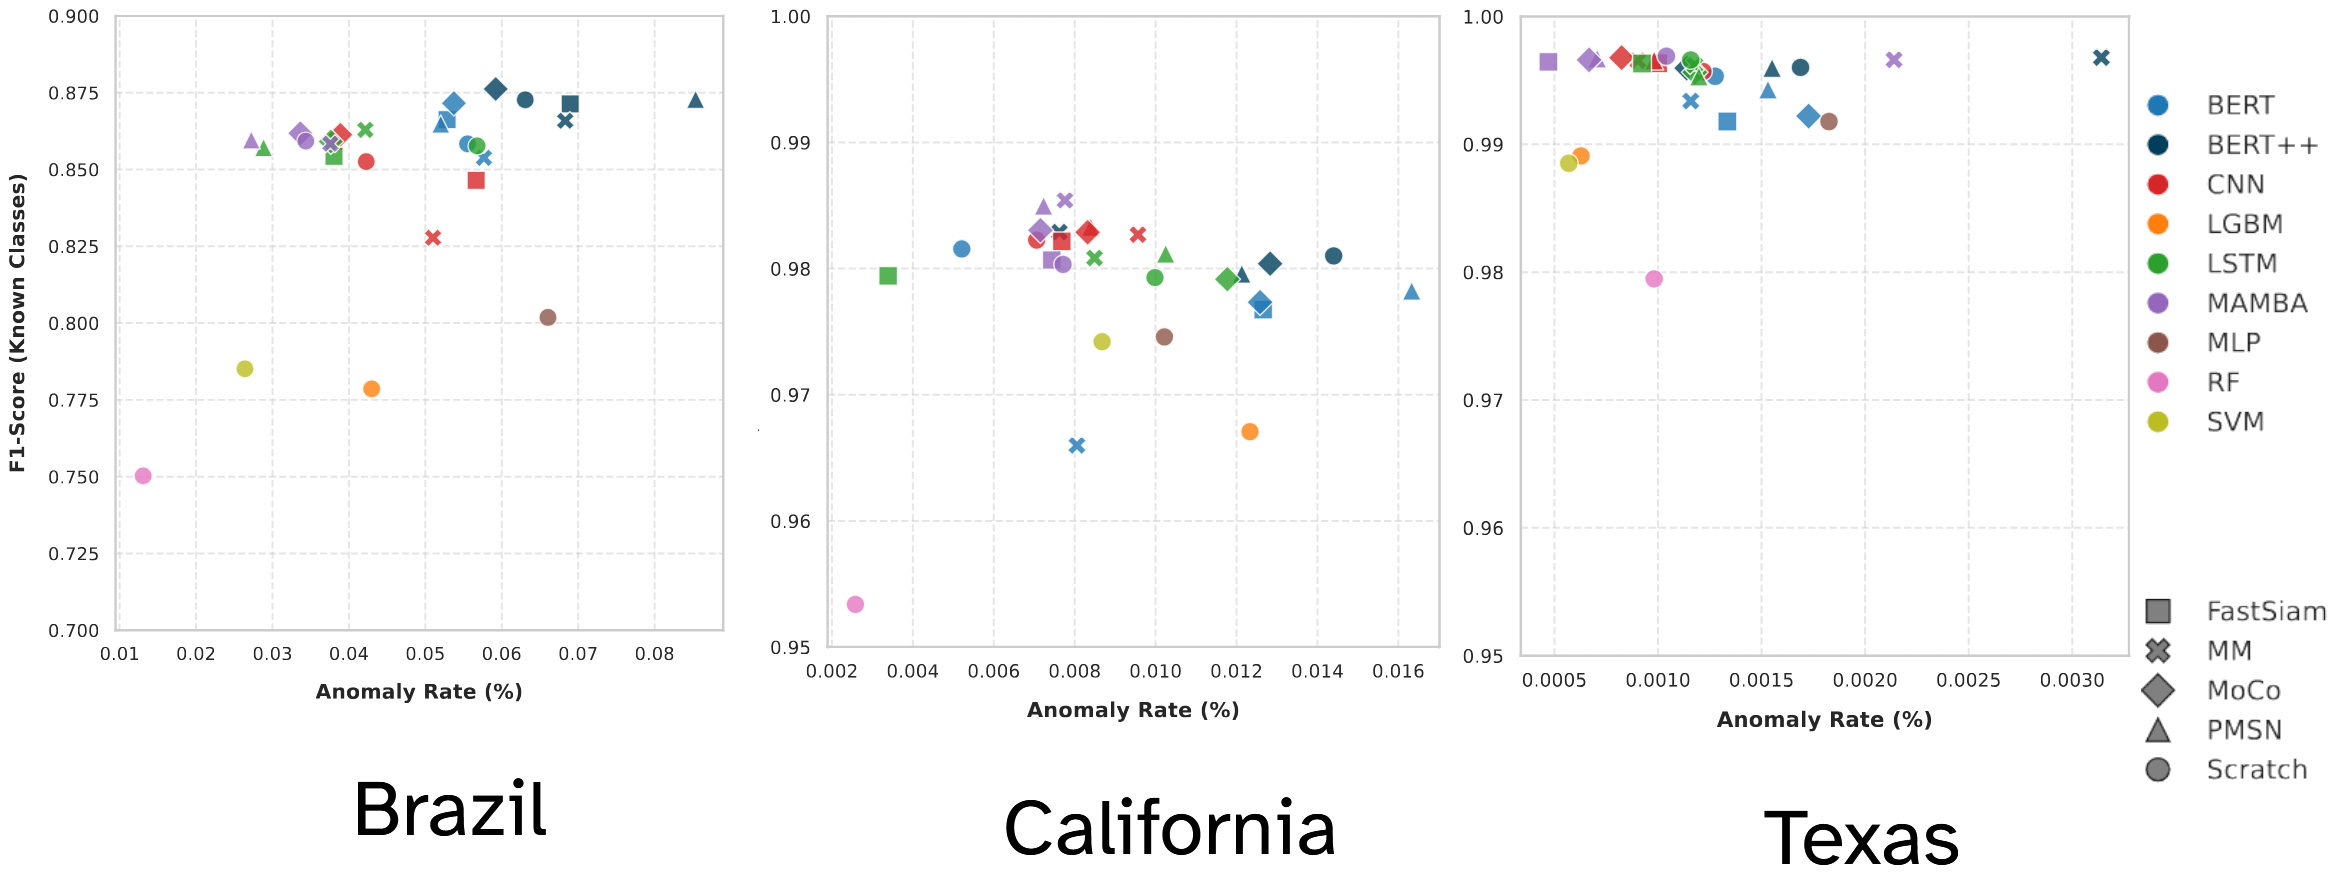
\includegraphics[width=\textwidth, keepaspectratio]{figures_slides/order_slides.jpg}
    \end{figure}

\end{frame}

\subsection{Best Results per Dataset}

\begin{frame}{Best Setup: Brazil Dataset}
    \begin{block}{SITS-BERT++ (MoCo Pre-training)}
        The proposed ORDER framework achieves a distinct bimodal separation between correct and incorrect predictions for crops like Citrus and Coffee.
    \end{block}
    
    \vspace{0.2cm}
    
    \begin{figure}
        \centering
        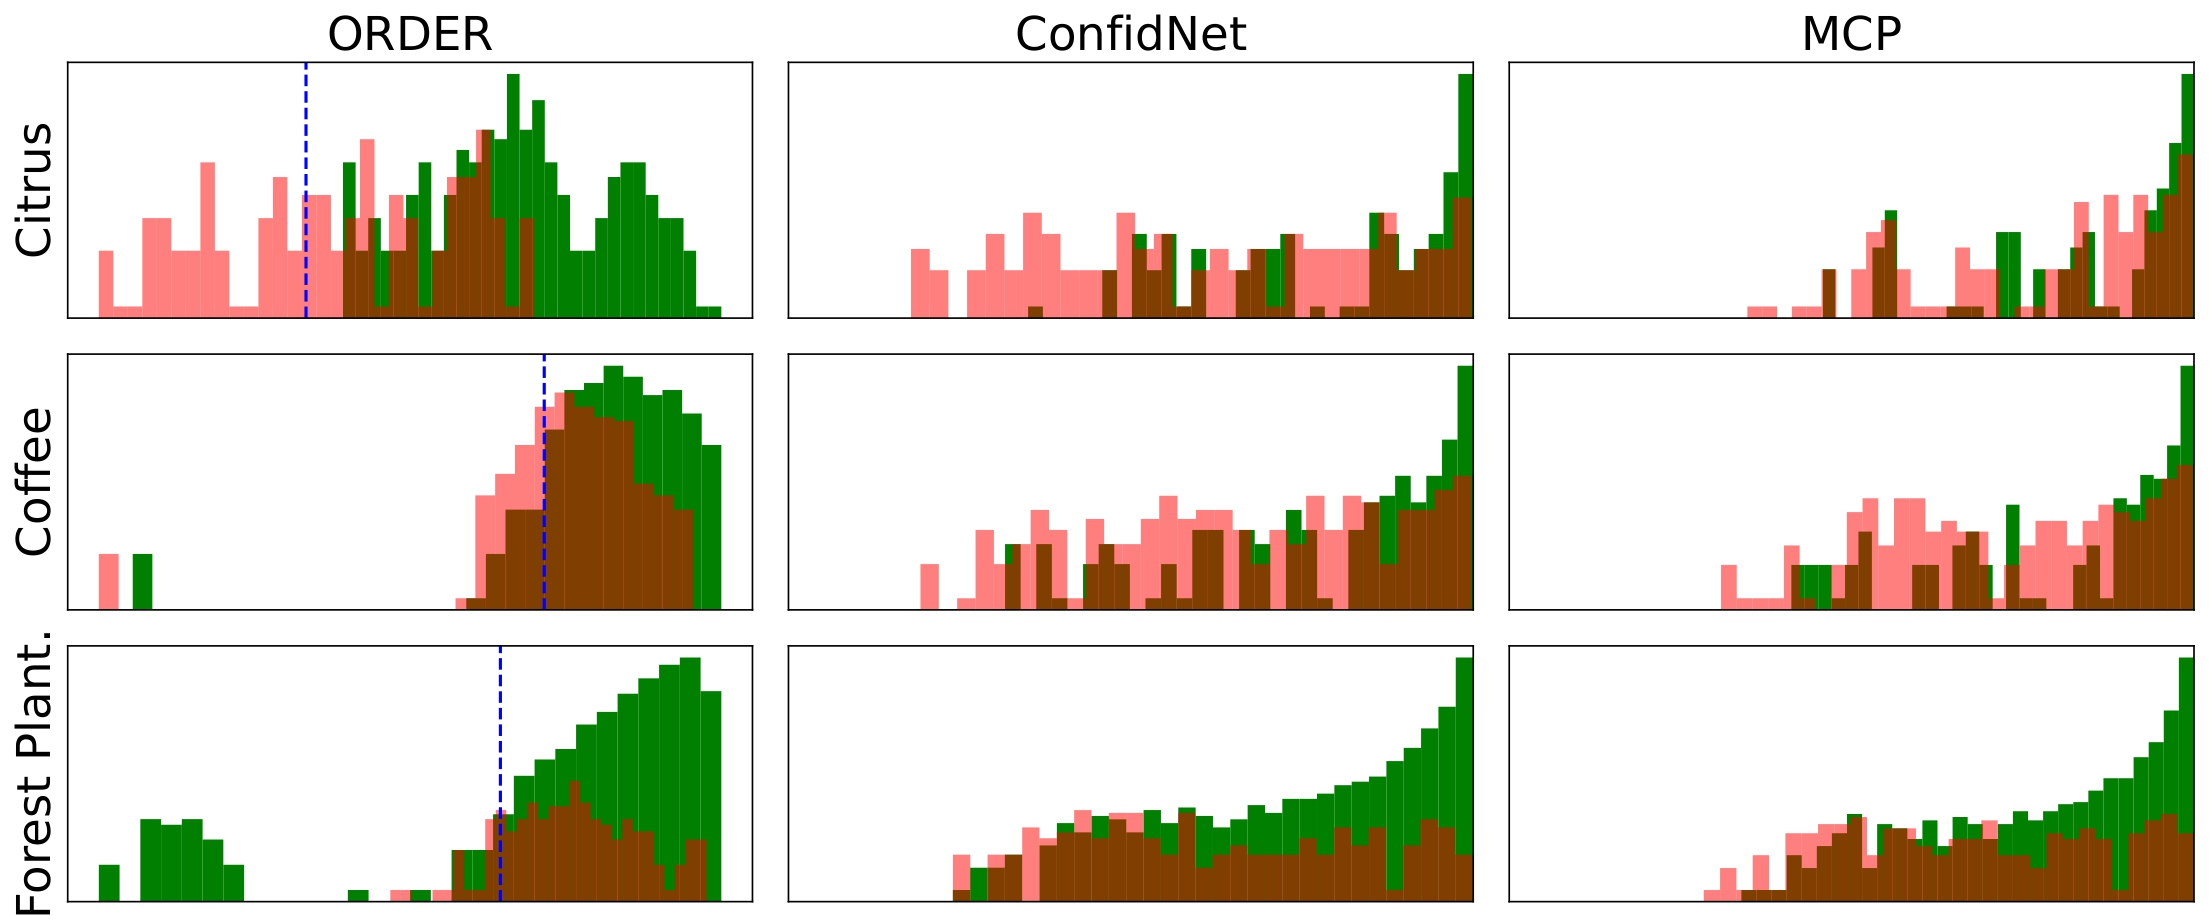
\includegraphics[height=0.41\textheight, width=\textwidth, keepaspectratio]{figures_slides/hist_combined_brasil.jpg}
    \end{figure}

\end{frame}

\section{Conclusion}
\label{sec:08:conclusion}

\begin{frame}{Concluding Remarks: General Summary}
    \begin{block}{A Data-Centric Lightweight Pipeline}
        This work explored a scalable pipeline for parcel-level crop classification using public labels and Sentinel-2 data. The DCAI filtering strategy allowed the creation of datasets even from noisy public sources.
    \end{block}

    \pause

    \begin{block}{Models \& Reliability}
        \begin{itemize}
            \item Deep Learning models generally showed better performance than Shallow baselines, particularly in complex scenarios like Brazil.
            \item Self-Supervised Learning indicated a positive impact as a regularizer in data-scarce regimes.
            \item The proposed \textbf{ORDER} method demonstrated promising potential in separating correct from incorrect predictions, offering a viable alternative to mitigate model overconfidence.
        \end{itemize}
    \end{block}
\end{frame}

\begin{frame}{Answering RQ5: Anomaly Detection (ORDER)}
    \begin{block}{Research Question 5}
        Is it possible to improve confidence estimation or detect model anomalies through generative models on embeddings, surpassing established baselines such as ConfidNet?
    \end{block}

    \begin{block}{Conclusion}
        \begin{itemize}
            \item Detecting anomalies during prediction using embedding analysis methods like \textbf{ORDER} proved to be a viable strategy.
            \item \textbf{ORDER} generated a visually clearer bimodal differentiation between correct and incorrect predictions compared to the ConfidNet baseline and the standard Maximum Class Probability (MCP).
            \item While formal confidence ranking was not fully explored, the well-behaved prediction scores suggest it is a promising avenue for future work.
        \end{itemize}
    \end{block}
\end{frame}

\begin{frame}
    \begin{center}
        
\includegraphics[height=1.2cm]{logos_institutos/logo_ibge.png} \hspace{0.5cm}
        
\includegraphics[height=1.2cm]{logos_institutos/logo_mavilab.png} \hspace{0.5cm}
        
\includegraphics[height=1.2cm]{logos_institutos/logo_patreo.png} \hspace{0.5cm}
        
\includegraphics[height=1.2cm]{logos_institutos/logo_serrapilheira.png}
    \end{center}
    
    \vspace{0.5cm} 
    
    \begin{center}
        \LARGE{\textbf{Thank You!}} \\
        \vspace{0.8cm}
        \large{Mateus Pinto da Silva} \\
        \vspace{0.2cm}
        \normalsize{\textit{Universidade Federal de Viçosa (UFV)}} \\
        \vspace{0.8cm}
        \normalsize{\textbf{Questions?}}
    \end{center}
    
    \vfill
    
    \begin{flushleft}
        \tiny{Contact: mateus.p.silva@ufv.br \\
        Registration Code: EF3489}
    \end{flushleft}
\end{frame}

\end{document}